\section{Exercice 11 - Coloration des sommets d'un graphe et coloration des arêtes d'un graphe}

Un graphe est $2-$coloriable si et seulement si il est possible de partitionner ce dernier en deux
ensembles stables. Un graphe 2-coloriable est donc un graphe biparti, or le problème de décider si
un graphe est biparti est un problème polynomial, le problème de la $2-$coloration est donc un
problème polynomial.

Un graphe est $2-$arête$-$coloriable s'il l'ensemble $V$ de ses arêtes est divisible en deux ensembles
$F$ et $E$ distincts vérifiant :
\begin{enumerate}
	\item $E \cup F = V$
	\item $E \cap F = \emptyset$
	\item $\forall ((i,j), (k,l)) \in E^2, \quad i \not = k, \not = l, j \not = k, j \not = l$
	\item $\forall ((i,j), (k,l)) \in J^2, \quad i \not = k, \not = l, j \not = k, j \not = l$
\end{enumerate}

$E$ et $F$ sont alors des couplages de $G$. Un algorithme résolvant ce problème consiste en la
recherche d'un couplage maximum $C$ puis en vérifiant que $V \ C$ est aussi un couplage. Si tel est
le cas, le graphe est $2-$arête$-$coloriable. 

La recherche d'un couplage se faisant en temps polynomial, l'algorithme énoncé ci-dessus est
polynomial.

\section{Exercice 12 - Coloration des sommets d'un graphe}

\subsection{Appartenance à $NP$}

\begin{enumerate}
	\item COLOR : \\
		Considérons une solution, un moyen de tester s'il s'agit d'une solution réalisable est de tester
		pour chacun des sommets si ses voisins sont d'une couleur différente en gardant le s couleurs
		rencontrées en mémoire afin de vérifier que leur nombre n'excède pas $k$. La vérification se
		fait alors en $O(n^2)$ et est donc polynomiale.
	\item 3-COLOR : \\
		On procède de la même manière que pour COLOR en s'assurant que le nombre de couleur ne dépasse
		pas $3$, la vérification est alors aussi polynomiale
	\item 3-COLOR-PLAN : \\
		La vérification de la validité de la $3-$coloration se fait comme précédemment en $O(n^2)$. Il
		fait cependant tester si le graphe est planaire qui est un problème polynomial, la vérification
		est don cpolynomiale.
\end{enumerate}

Tous ces problèmes appartiennent donc à $NP$.

\subsection{Relation enre 3-COLOR et COLOR}

Supposons qu'il existe un algorithme résolvant COLOR en temps polynomial quelque soit $k$, il existe
alors un algorithme polynomial résolvant 3-COLOR. Par contraposition, on vient de démontrer que si
3-COLOR est $NP$-difficile alors COLOR est $NP$-difficile.

\subsection{Étude du problème COLOR}

\subsubsection{Graphe $G_{\phi}$}


\begin{center}
	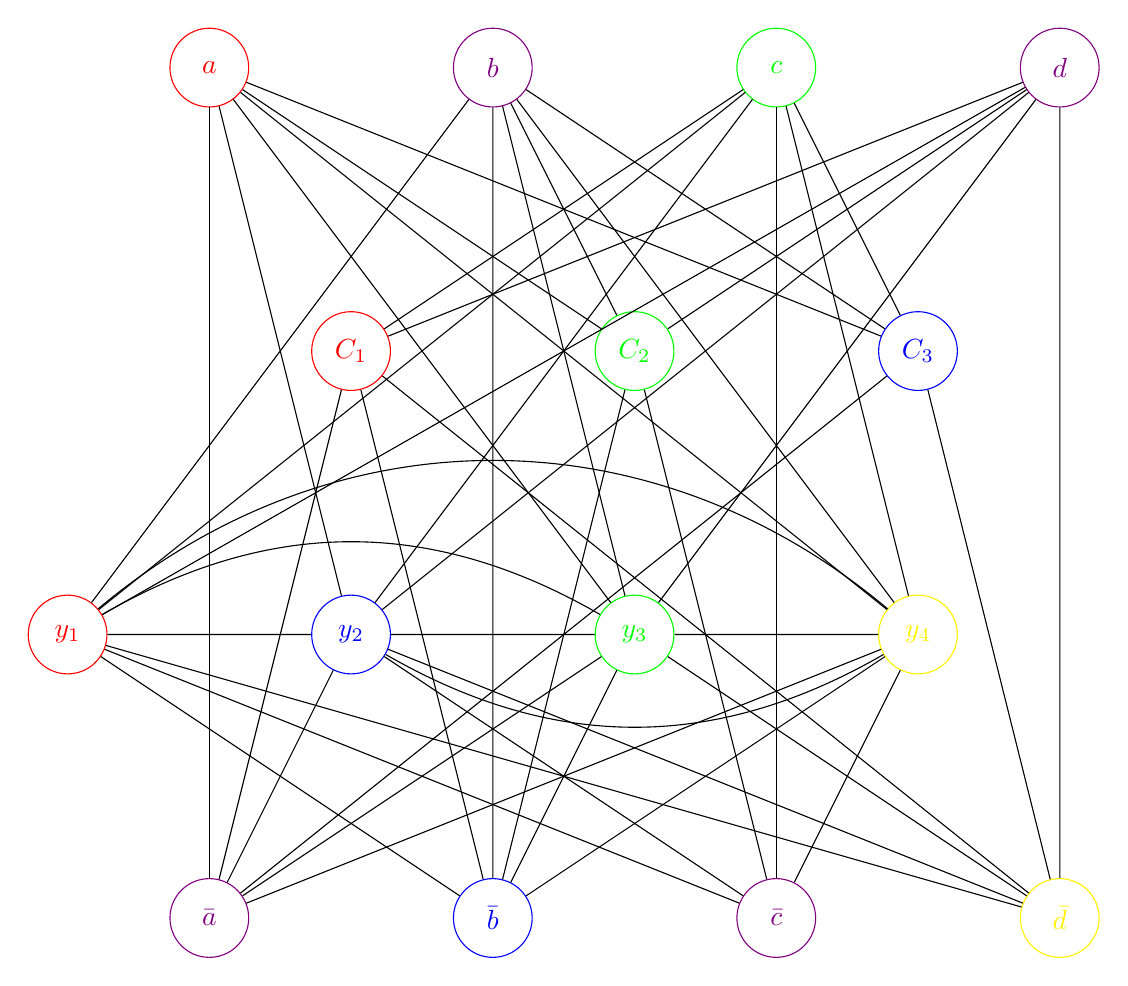
\begin{tikzpicture}[scale=1.8]
		\tikzset{nd/.style={circle, draw=black, minimum width=1cm}};
		\node[nd, red] (a) at (2, 6) {$a$};
		\node[nd, violet] (b) at (4, 6) {$b$};
		\node[nd, green] (c) at (6, 6) {$c$};
		\node[nd, violet] (d) at (8, 6) {$d$};
		\node[nd, violet] (na) at (2, 0) {$\bar a$};
		\node[nd, blue] (nb) at (4, 0) {$\bar b$};
		\node[nd, violet] (nc) at (6, 0) {$\bar c$};
		\node[nd, yellow] (nd) at (8, 0) {$\bar d$};
		\node[nd, red] (c1) at (3, 4) {$C_1$};
		\node[nd, green] (c2) at (5, 4) {$C_2$};
		\node[nd, blue] (c3) at (7, 4) {$C_3$};
		\node[nd, red] (y1) at (1, 2) {$y_1$};
		\node[nd, blue] (y2) at (3, 2) {$y_2$};
		\node[nd, green] (y3) at (5, 2) {$y_3$};
		\node[nd, yellow] (y4) at (7, 2) {$y_4$};

		\draw (a) -- (na);
		\draw (b) -- (nb);
		\draw (c) -- (nc);
		\draw (d) -- (nd);

		\draw (y1) -- (y2);
		\draw (y1) to[out=30, in=150](y3);
		\draw (y1) to[out=40, in=140](y4);

		\draw (y2) -- (y3);
		\draw (y2) to[out=330, in=210] (y4);

		\draw (y3) -- (y4);

		\draw (y1) -- (b);
		\draw (y1) -- (c);
		\draw (y1) -- (d);
		\draw (y1) -- (nb);
		\draw (y1) -- (nc);
		\draw (y1) -- (nd);

		\draw (y2) -- (a);
		\draw (y2) -- (c);
		\draw (y2) -- (d);
		\draw (y2) -- (na);
		\draw (y2) -- (nc);
		\draw (y2) -- (nd);

		\draw (y3) -- (a);
		\draw (y3) -- (b);
		\draw (y3) -- (d);
		\draw (y3) -- (na);
		\draw (y3) -- (nb);
		\draw (y3) -- (nd);

		\draw (y4) -- (a);
		\draw (y4) -- (b);
		\draw (y4) -- (c);
		\draw (y4) -- (na);
		\draw (y4) -- (nb);
		\draw (y4) -- (nc);

		\draw (c1) -- (na);
		\draw (c1) -- (nb);
		\draw (c1) -- (c);
		\draw (c1) -- (d);
		\draw (c1) -- (nd);

		\draw (c2) -- (a);
		\draw (c2) -- (nb);
		\draw (c2) -- (nc);
		\draw (c2) -- (d);
		\draw (c2) -- (b);

		\draw (c3) -- (na);
		\draw (c3) -- (a);
		\draw (c3) -- (b);
		\draw (c3) -- (c);
		\draw (c3) -- (nd);


	\end{tikzpicture}
\end{center}


\subsubsection{$\phi$ satisfiable $\Rightarrow$ $n+1-$coloration de $G_\phi$}

Nous allons chercher à montrer que la coloration donnée est une coloration valide.
Prenons les différents points un à un : 
\begin{itemize}
	\item les $y_i$ sont reliés les uns avec les autres mais sont tous de couleur différente, et ils
		sont reliés aux $x_j et \bar x_j$ tels que $i \not = j$, or ces derniers sont soit de la couleur
		$j$, donc différente de la couleur $i$, soit de la couleur $n+1$ donc différente aussi
	\item les $C_k$ sont de la couleur d'un des $x_i$ la satisfaisant et sont reliés aux $x_j$ et
		$\bar x_j$ n'apparaissant pas dans cette dernière, or ces derniers sont soit de couleur $n+1$
		soit de couleur $j$ différente de la couleur de $C_k$\footnote{Imaginons qu'un des $x_j$ soit de
			la couleur de $C_k$, ceci n'est possible que si $j = i$ et donc que si le n\oe ud $\x_i = \bar
			x_j$, or si $x_i$ a donné sa couleur à $C_k$ c'est qu'il satisfait cette dernière et donc que
		$x_j$ est de couleur $n+1$, il ne peut donc pas être de la même couleur que $C_k$ }.
	\item les $x_i$ sont reliés aux $\bar x_i$, or si un $x_i$ est de couleur $i$, $\bar x_i$ est de
		couleur $n+1$ et vice-versa, ils sont donc d'une couleur différente
\end{itemize}

Nous avons passé en revue l'ensemble des arêtes de $G_\phi$ sans trouver de failles, une solution de
$\phi$ nous donne une coloration de $G_\phi$.

\subsubsection{Couleurs des $y_i$}

Tous les $y_i$ sont adjacents les uns aux autres, ils forment alors un graphe complet. Or le nombre
chromatique d'un graphe complet à $n$ sommets et $n$ et tous les sommets ont des couleurs
différentes. Donc si le graphe est $n+1-$colorié, tous les $y_i$ ont une couleur différente.

\subsubsection{Couleurs des $C_k$}

Le nombre de variables est supérieur à 3, donc il y a forcément au moins une variable n'apparaissant
pas dans la clause $k^e$ clause, nous appellerons $x_i$ l'une de ces variables. Par définition $x_i$
et $\bar x_i$ sont reliés à $C_k$, or l'une des deux variables est de couleur $n+1$ donc $C_k$ ne
peut être de couleur $n+1$.

\subsubsection{$G_\phi$ $n+1-$coloriable $\Rightarrow$ $\phi$est satisfaisable}

\subsubsection{$NP$-complétude de COLOR}

\subsection{Étude de 3-COLOR}

\subsubsection{Construction du graphe}

\begin{center}
\begin{tikzpicture}
\tikzset{nd/.style={circle, draw=black, minimum size=1cm}};


\end{tikzpicture}
\end{center}


\subsubsection{$\phi \in$ NAE-3-SAT $ \Rightarrow $ 3-coloration de $G_\phi$}

Nous allons cherhcer à démontrer que la coloration obtenue est une coloration valide. pour ce faire,
prenons les différents points un à un :
\begin{itemize}
	\item les $x_i$ sont reliés au $\bar x_i$, or si $x_i$ est vraie le sommet est coloré en rouge,
		$\bar x_i$ est alors coloré en noir et inversement. Les deux n'ont donc pas la même couleur.
	\item $V$, coloré en vert, est rélié aux variables, colorées en rouge ou en noir. Les sommets
		n'ont donc pas la même couleur
	\item utilisons, pour les triangles de clauses, le fait que $\phi \in$ NAE-3-SAT. Ceci indique
		qu'à lintérieur d'une même clause, toutes les variables ne peuvent avoir la même valeur. On aura
		donc, quelque soit le cas, un sommet du triangle relié à une variable colorée en noir
		(respectivement rouge) et les autres sommets du triangle reliés à des variables colorées en
		rouge (respectivement noir). Chaque sommet du triangle est alors relié à trois sommets dont les
		couleurs sont différentes de la sienne.
\end{itemize}

Il s'agit alors d'une coloration valide.

\subsubsection{Les triangles de clauses}

Supposons $G_\phi$ coloré avec 3 couleurs et supposons que l'un des triangles de clauses soit relié
à trois sommets de couleur identique. Le triangle étant un graphe complet de taille 3, le nombre de
couleurs pour le colorer est de 3, si la couleur des trois sommets reliés au triangle est rouge, le
sommet du triangle de couleur rouge sera relié à un sommet rouge, il ne s'agit alors plus d'une
coloration valide. On peut faire le même raisonnement
sur le vert et le noir. Les trois sommets reliés au triangle ne peuvent être de couleur identique.

De plus, le fait que $V$ soit coloré en vert et relié à chacune des variables imposent à ces
dernières d'être soit noires, soit rouges. Et donc le triangle est relié à au moins un littéral de
couleur noire et au moins un de couleur rouge.

\subsection{3-COLOR-PLAN}

\subsubsection{Couleur des sommets deux à deux}

Nous allons montrer qu'il n'existe qu'une seule manière de colorer ce graphe avec $3$
couleurs\footnote{à permutation des couleurs près}. Pour ce faire commençons par rermarquer que
chaque point appartient à au moins une clique de taille trois, ce qui impose la couleur de ses
voisins. Donc quelques soit le point de départ, il existera une unique façon de colorer les voisins
de ce point appartenant à la clique de taille 3, eux même imposant la couleur de leur voisin et
ainsi de suite. 
Afin de démontrer l'imossibilité de colorer d'une autre manière nous ne réaliserons aucune
coloration arbitraire de n\oe ud, si ce n'est la coloration initiale. Commençons donc par le point
$A$ coloré en rouge. Ce dernier appartien à une clique de taille $3$ avec les sommets $1$ et $2$,
ils doivent donc avoir une couleur différente, $1$ sera bleu et $2$ sera vert. 

\begin{center}
	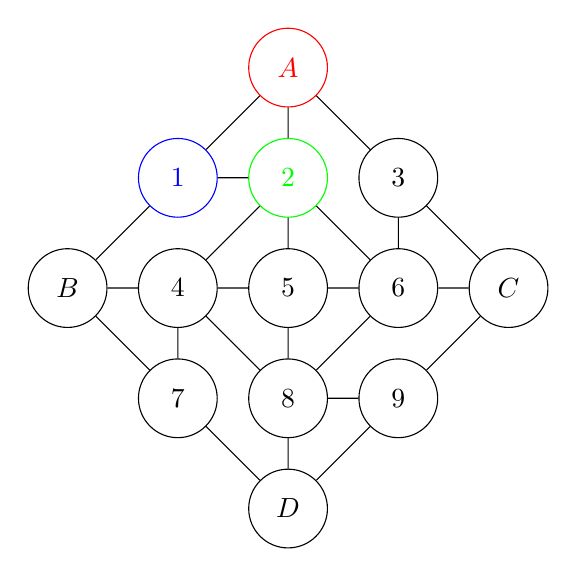
\begin{tikzpicture}[scale=1.4]
		\tikzset{nd/.style={circle, draw=black, minimum width=1cm}};

		\node[nd, red] (a) at (2, 4) {$A$};
		\node[nd, blue] (1) at (1, 3) {$1$};
		\node[nd, green] (2) at (2, 3) {$2$};
		\node[nd] (3) at (3, 3) {$3$};
		\node[nd] (b) at (0, 2) {$B$};
		\node[nd] (4) at (1, 2) {$4$};
		\node[nd] (5) at (2, 2) {$5$};
		\node[nd] (6) at (3, 2) {$6$};
		\node[nd] (c) at (4, 2) {$C$};
		\node[nd] (7) at (1, 1) {$7$};
		\node[nd] (8) at (2, 1) {$8$};
		\node[nd] (9) at (3, 1) {$9$};
		\node[nd] (d) at (2, 0) {$D$};

		\draw (a) to (1);
		\draw (a) to (2);
		\draw (a) to (3);

		\draw (1) to (2);
		\draw (1) to (b);

		\draw (2) to (4);
		\draw (2) to (5);
		\draw (2) to (6);

		\draw (3) to (6);
		\draw (3) to (c);

		\draw (b) to (4);
		\draw (b) to (7);

		\draw (4) to (5);
		\draw (4) to (7);
		\draw (4) to (8);

		\draw (5) to (8);
		\draw (5) to (6);

		\draw (6) to (c);
		\draw (6) to (8);

		\draw (c) to (9);

		\draw (7) to (d);
		
		\draw (8) to (d);
		\draw (8) to (9);

		\draw (9) to (d);
	\end{tikzpicture}
\end{center}


On voi alors que $2$ appartient à deux cliques de taille 3, on colore donc ces dernières.

\begin{center}
	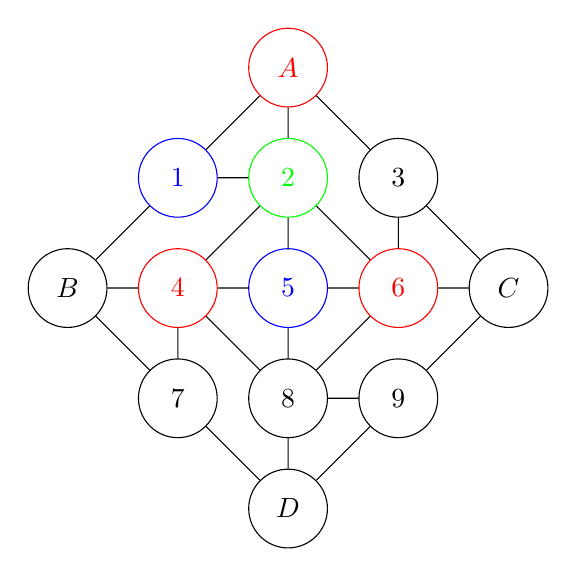
\begin{tikzpicture}[scale=1.4]
		\tikzset{nd/.style={circle, draw=black, minimum width=1cm}};

		\node[nd, red] (a) at (2, 4) {$A$};
		\node[nd, blue] (1) at (1, 3) {$1$};
		\node[nd, green] (2) at (2, 3) {$2$};
		\node[nd] (3) at (3, 3) {$3$};
		\node[nd] (b) at (0, 2) {$B$};
		\node[nd, red] (4) at (1, 2) {$4$};
		\node[nd, blue] (5) at (2, 2) {$5$};
		\node[nd, red] (6) at (3, 2) {$6$};
		\node[nd] (c) at (4, 2) {$C$};
		\node[nd] (7) at (1, 1) {$7$};
		\node[nd] (8) at (2, 1) {$8$};
		\node[nd] (9) at (3, 1) {$9$};
		\node[nd] (d) at (2, 0) {$D$};

		\draw (a) to (1);
		\draw (a) to (2);
		\draw (a) to (3);

		\draw (1) to (2);
		\draw (1) to (b);

		\draw (2) to (4);
		\draw (2) to (5);
		\draw (2) to (6);

		\draw (3) to (6);
		\draw (3) to (c);

		\draw (b) to (4);
		\draw (b) to (7);

		\draw (4) to (5);
		\draw (4) to (7);
		\draw (4) to (8);

		\draw (5) to (8);
		\draw (5) to (6);

		\draw (6) to (c);
		\draw (6) to (8);

		\draw (c) to (9);

		\draw (7) to (d);
		
		\draw (8) to (d);
		\draw (8) to (9);

		\draw (9) to (d);
	\end{tikzpicture}
\end{center}


Le sommet $5$ appartient à une clique, et le sommet $B$ n'a qu'une seule couleur possible, on
réalise donc les colorations nécessaires.

\begin{center}
	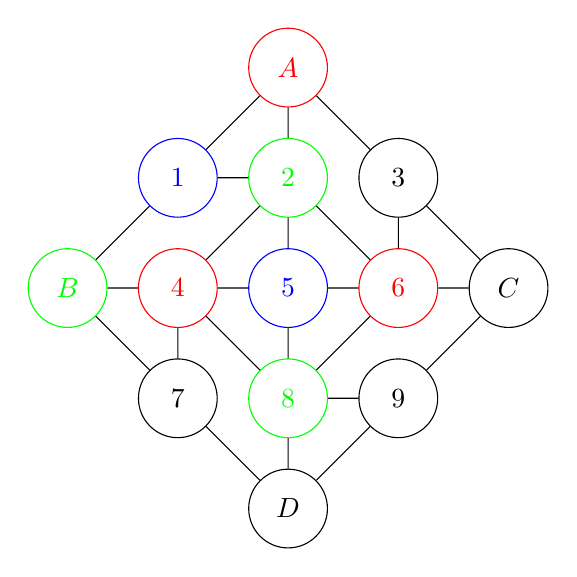
\begin{tikzpicture}[scale=1.4]
		\tikzset{nd/.style={circle, draw=black, minimum width=1cm}};

		\node[nd, red] (a) at (2, 4) {$A$};
		\node[nd, blue] (1) at (1, 3) {$1$};
		\node[nd, green] (2) at (2, 3) {$2$};
		\node[nd] (3) at (3, 3) {$3$};
		\node[nd, green] (b) at (0, 2) {$B$};
		\node[nd, red] (4) at (1, 2) {$4$};
		\node[nd, blue] (5) at (2, 2) {$5$};
		\node[nd, red] (6) at (3, 2) {$6$};
		\node[nd] (c) at (4, 2) {$C$};
		\node[nd] (7) at (1, 1) {$7$};
		\node[nd, green] (8) at (2, 1) {$8$};
		\node[nd] (9) at (3, 1) {$9$};
		\node[nd] (d) at (2, 0) {$D$};

		\draw (a) to (1);
		\draw (a) to (2);
		\draw (a) to (3);

		\draw (1) to (2);
		\draw (1) to (b);

		\draw (2) to (4);
		\draw (2) to (5);
		\draw (2) to (6);

		\draw (3) to (6);
		\draw (3) to (c);

		\draw (b) to (4);
		\draw (b) to (7);

		\draw (4) to (5);
		\draw (4) to (7);
		\draw (4) to (8);

		\draw (5) to (8);
		\draw (5) to (6);

		\draw (6) to (c);
		\draw (6) to (8);

		\draw (c) to (9);

		\draw (7) to (d);
		
		\draw (8) to (d);
		\draw (8) to (9);

		\draw (9) to (d);
	\end{tikzpicture}
\end{center}


La couleur du sommet $7$ est obligatoirement bleue, ce qui obliqe $D$ à être rouge, puis $9$ à être
bleu, $C$ vert et enfin $3$ bleu.

\begin{center}
	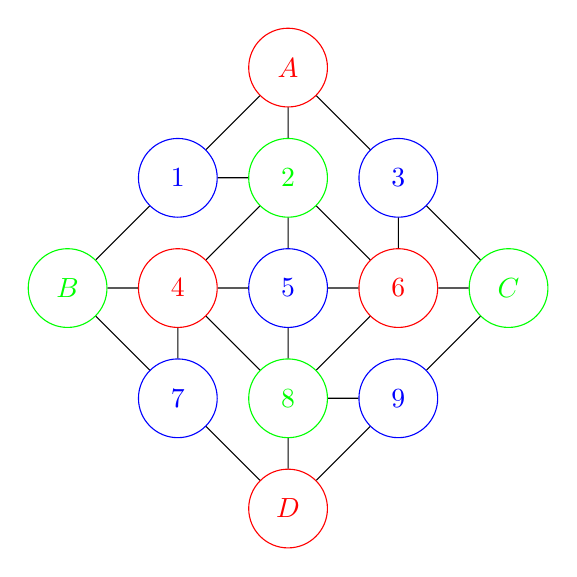
\begin{tikzpicture}[scale=1.4]
		\tikzset{nd/.style={circle, draw=black, minimum width=1cm}};

		\node[nd, red] (a) at (2, 4) {$A$};
		\node[nd, blue] (1) at (1, 3) {$1$};
		\node[nd, green] (2) at (2, 3) {$2$};
		\node[nd, blue] (3) at (3, 3) {$3$};
		\node[nd, green] (b) at (0, 2) {$B$};
		\node[nd, red] (4) at (1, 2) {$4$};
		\node[nd, blue] (5) at (2, 2) {$5$};
		\node[nd, red] (6) at (3, 2) {$6$};
		\node[nd, green] (c) at (4, 2) {$C$};
		\node[nd, blue] (7) at (1, 1) {$7$};
		\node[nd, green] (8) at (2, 1) {$8$};
		\node[nd, blue] (9) at (3, 1) {$9$};
		\node[nd, red] (d) at (2, 0) {$D$};

		\draw (a) to (1);
		\draw (a) to (2);
		\draw (a) to (3);

		\draw (1) to (2);
		\draw (1) to (b);

		\draw (2) to (4);
		\draw (2) to (5);
		\draw (2) to (6);

		\draw (3) to (6);
		\draw (3) to (c);

		\draw (b) to (4);
		\draw (b) to (7);

		\draw (4) to (5);
		\draw (4) to (7);
		\draw (4) to (8);

		\draw (5) to (8);
		\draw (5) to (6);

		\draw (6) to (c);
		\draw (6) to (8);

		\draw (c) to (9);

		\draw (7) to (d);
		
		\draw (8) to (d);
		\draw (8) to (9);

		\draw (9) to (d);
	\end{tikzpicture}
\end{center}


L'unicité de cette coloration (à permutation près) est sue à l'unicité de la coloration du sous
graphe formé par les sommets $2$, $4$, $5$, $6$ et $8$.
Et on a bien les couleur de $A$ et $D$ (respectivement $B$ et $C$) appareillée.

\subsubsection{Coloration avec les couleurs des extrêmités données}

Comme annoncé précédemment, lorsque les couleurs  sont fixées, il n'y a plus de choix possibles,
toutes les possibilités de coloration sont fixées.

Prenons un nouvel exemple, le cas ou $A$ et $B$ sont de couleur différente ayant été présenté
précédemment, nous et fixons $A$, $B$, $C$ et $D$ à rouge.

\begin{center}
	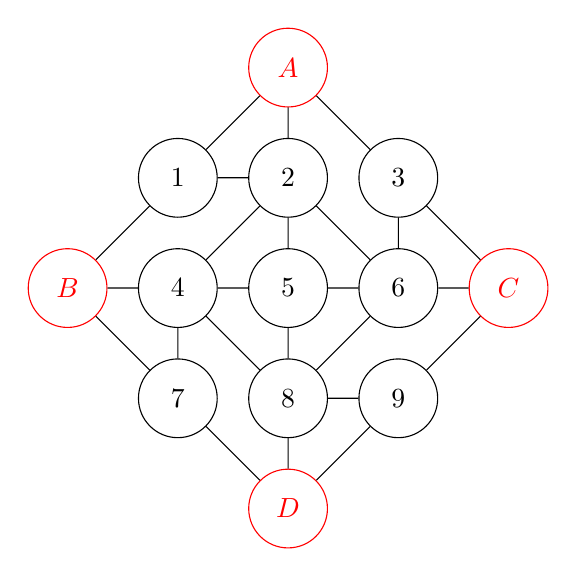
\begin{tikzpicture}[scale=1.4]
		\tikzset{nd/.style={circle, draw=black, minimum width=1cm}};

		\node[nd, red] (a) at (2, 4) {$A$};
		\node[nd] (1) at (1, 3) {$1$};
		\node[nd] (2) at (2, 3) {$2$};
		\node[nd] (3) at (3, 3) {$3$};
		\node[nd, red] (b) at (0, 2) {$B$};
		\node[nd] (4) at (1, 2) {$4$};
		\node[nd] (5) at (2, 2) {$5$};
		\node[nd] (6) at (3, 2) {$6$};
		\node[nd, red] (c) at (4, 2) {$C$};
		\node[nd] (7) at (1, 1) {$7$};
		\node[nd] (8) at (2, 1) {$8$};
		\node[nd] (9) at (3, 1) {$9$};
		\node[nd, red] (d) at (2, 0) {$D$};

		\draw (a) to (1);
		\draw (a) to (2);
		\draw (a) to (3);

		\draw (1) to (2);
		\draw (1) to (b);

		\draw (2) to (4);
		\draw (2) to (5);
		\draw (2) to (6);

		\draw (3) to (6);
		\draw (3) to (c);

		\draw (b) to (4);
		\draw (b) to (7);

		\draw (4) to (5);
		\draw (4) to (7);
		\draw (4) to (8);

		\draw (5) to (8);
		\draw (5) to (6);

		\draw (6) to (c);
		\draw (6) to (8);

		\draw (c) to (9);

		\draw (7) to (d);
		
		\draw (8) to (d);
		\draw (8) to (9);

		\draw (9) to (d);
	\end{tikzpicture}
\end{center}


Le sommet $5$ est obligatoirement rouge lui aussi.

\begin{center}
	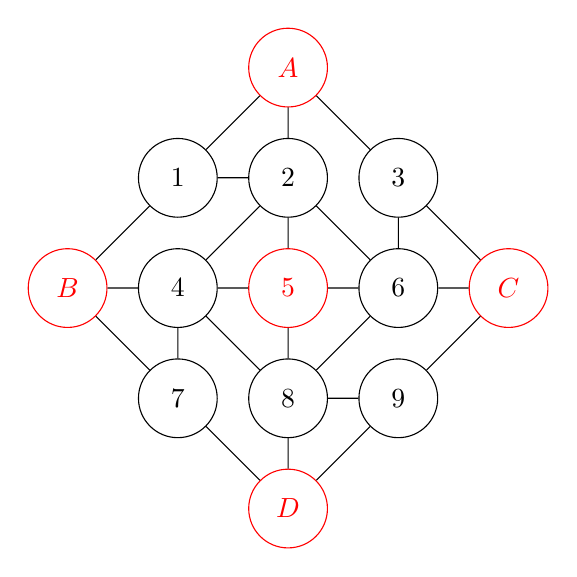
\begin{tikzpicture}[scale=1.4]
		\tikzset{nd/.style={circle, draw=black, minimum width=1cm}};

		\node[nd, red] (a) at (2, 4) {$A$};
		\node[nd] (1) at (1, 3) {$1$};
		\node[nd] (2) at (2, 3) {$2$};
		\node[nd] (3) at (3, 3) {$3$};
		\node[nd, red] (b) at (0, 2) {$B$};
		\node[nd] (4) at (1, 2) {$4$};
		\node[nd, red] (5) at (2, 2) {$5$};
		\node[nd] (6) at (3, 2) {$6$};
		\node[nd, red] (c) at (4, 2) {$C$};
		\node[nd] (7) at (1, 1) {$7$};
		\node[nd] (8) at (2, 1) {$8$};
		\node[nd] (9) at (3, 1) {$9$};
		\node[nd, red] (d) at (2, 0) {$D$};

		\draw (a) to (1);
		\draw (a) to (2);
		\draw (a) to (3);

		\draw (1) to (2);
		\draw (1) to (b);

		\draw (2) to (4);
		\draw (2) to (5);
		\draw (2) to (6);

		\draw (3) to (6);
		\draw (3) to (c);

		\draw (b) to (4);
		\draw (b) to (7);

		\draw (4) to (5);
		\draw (4) to (7);
		\draw (4) to (8);

		\draw (5) to (8);
		\draw (5) to (6);

		\draw (6) to (c);
		\draw (6) to (8);

		\draw (c) to (9);

		\draw (7) to (d);
		
		\draw (8) to (d);
		\draw (8) to (9);

		\draw (9) to (d);
	\end{tikzpicture}
\end{center}


On a alors $2$ et $8$ de même couleur, ainsi que $4$ et $6$ et $2$ et $4$ de couleur différente.

\begin{center}
	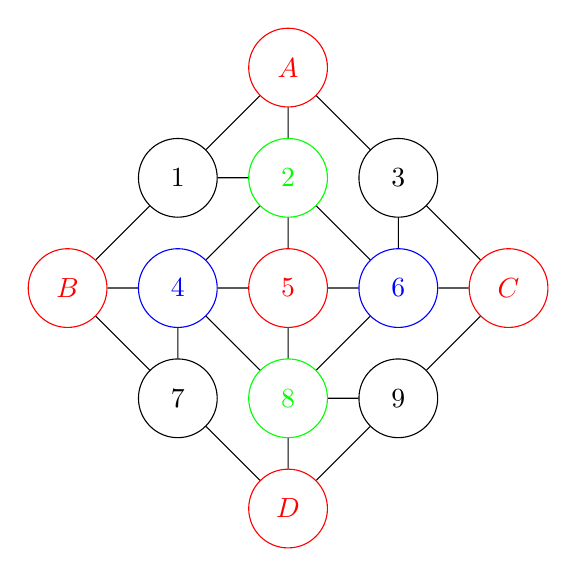
\begin{tikzpicture}[scale=1.4]
		\tikzset{nd/.style={circle, draw=black, minimum width=1cm}};

		\node[nd, red] (a) at (2, 4) {$A$};
		\node[nd] (1) at (1, 3) {$1$};
		\node[nd, green] (2) at (2, 3) {$2$};
		\node[nd] (3) at (3, 3) {$3$};
		\node[nd, red] (b) at (0, 2) {$B$};
		\node[nd, blue] (4) at (1, 2) {$4$};
		\node[nd, red] (5) at (2, 2) {$5$};
		\node[nd, blue] (6) at (3, 2) {$6$};
		\node[nd, red] (c) at (4, 2) {$C$};
		\node[nd] (7) at (1, 1) {$7$};
		\node[nd, green] (8) at (2, 1) {$8$};
		\node[nd] (9) at (3, 1) {$9$};
		\node[nd, red] (d) at (2, 0) {$D$};

		\draw (a) to (1);
		\draw (a) to (2);
		\draw (a) to (3);

		\draw (1) to (2);
		\draw (1) to (b);

		\draw (2) to (4);
		\draw (2) to (5);
		\draw (2) to (6);

		\draw (3) to (6);
		\draw (3) to (c);

		\draw (b) to (4);
		\draw (b) to (7);

		\draw (4) to (5);
		\draw (4) to (7);
		\draw (4) to (8);

		\draw (5) to (8);
		\draw (5) to (6);

		\draw (6) to (c);
		\draw (6) to (8);

		\draw (c) to (9);

		\draw (7) to (d);
		
		\draw (8) to (d);
		\draw (8) to (9);

		\draw (9) to (d);
	\end{tikzpicture}
\end{center}


Toutes les coueurs des autres n\oe uds sont alors fixées.

\begin{center}
	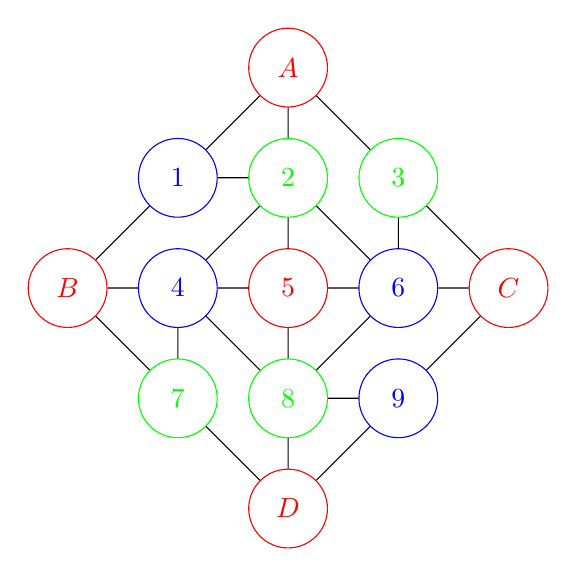
\begin{tikzpicture}[scale=1.4]
		\tikzset{nd/.style={circle, draw=black, minimum width=1cm}};

		\node[nd, red] (a) at (2, 4) {$A$};
		\node[nd, blue] (1) at (1, 3) {$1$};
		\node[nd, green] (2) at (2, 3) {$2$};
		\node[nd, green] (3) at (3, 3) {$3$};
		\node[nd, red] (b) at (0, 2) {$B$};
		\node[nd, blue] (4) at (1, 2) {$4$};
		\node[nd, red] (5) at (2, 2) {$5$};
		\node[nd, blue] (6) at (3, 2) {$6$};
		\node[nd, red] (c) at (4, 2) {$C$};
		\node[nd, green] (7) at (1, 1) {$7$};
		\node[nd, green] (8) at (2, 1) {$8$};
		\node[nd, blue] (9) at (3, 1) {$9$};
		\node[nd, red] (d) at (2, 0) {$D$};

		\draw (a) to (1);
		\draw (a) to (2);
		\draw (a) to (3);

		\draw (1) to (2);
		\draw (1) to (b);

		\draw (2) to (4);
		\draw (2) to (5);
		\draw (2) to (6);

		\draw (3) to (6);
		\draw (3) to (c);

		\draw (b) to (4);
		\draw (b) to (7);

		\draw (4) to (5);
		\draw (4) to (7);
		\draw (4) to (8);

		\draw (5) to (8);
		\draw (5) to (6);

		\draw (6) to (c);
		\draw (6) to (8);

		\draw (c) to (9);

		\draw (7) to (d);
		
		\draw (8) to (d);
		\draw (8) to (9);

		\draw (9) to (d);
	\end{tikzpicture}
\end{center}


\subsubsection{$NP$-complétude de 3-COLOR-PLAN}

Considéros un grapge $G$ et $H$ la transformation de $G$ réalisée de la sorte : pour tout couple
d'arêtes $(i,j)$ et $(k,l)$ s'intersectant de $G$, on insère au point d'intersection le graphe
étudié précédemment de sorte que $j$ soit confondu avec $C$, l'arête $(i,j)$ devient $(i, B)$, $l$
soit confondu avec $D$ et $(k,l)$ devient $(k,A)$.

Comme $A$ a la même couleur que $D$ (et donc que $j$), et que $B$ à la même couleur de $D$ (et donc
que $l$), on s'assure qu'une coloration valide pour $G$ est valide pour $H$. Ceci est vrai aussi
car il existe toujours une coloration du gadget pour une couleur fixée pour $A$ et $B$.

Supposons à présent qu'il existe une algorithme polynomial permettant de résoudre 3-COLOR-PLAN, la
transformation présentée ci dessus se faisant en $O(m^2)$, il existerait alors un algortihme
polynomial pour 3-COLOR. Or ce dernier est $NP$-difficile donc 3-COLOR-PLAN est aussi
$NP$-difficile.

\subsection{Restriction du problème 3-COLOR-PLAN}

\subsubsection{Exemple de coloration}

On fixe la couleur des sommets $A$, $B$ et $C$ à rouge.

\begin{center}
	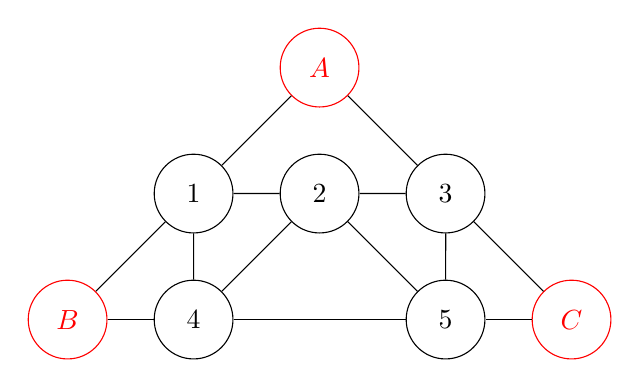
\begin{tikzpicture}[scale=1.6]
		\tikzset{nd/.style={circle, draw=black, minimum width=1cm}};

		\node[nd, red] (a) at (2, 2) {$A$};
		\node[nd] (1) at (1, 1) {$1$};
		\node[nd] (2) at (2, 1) {$2$};
		\node[nd] (3) at (3, 1) {$3$};
		\node[nd, red] (b) at (0, 0) {$B$};
		\node[nd] (4) at (1, 0) {$4$};
		\node[nd] (5) at (3, 0) {$5$};
		\node[nd, red] (c) at (4, 0) {$C$};

		\draw (a) to (1);
		\draw (a) to (3);

		\draw (1) to (2);
		\draw (1) to (b);
		\draw (1) to (4);

		\draw (2) to (3);
		\draw (2) to (4);
		\draw (2) to (5);

		\draw (3) to (5);
		\draw (3) to (c);

		\draw (b) to (4);

		\draw (4) to (5);

		\draw (5) to (c);


	\end{tikzpicture}
\end{center}


Le graphe est alors 3-coloriable : 

\begin{center}
	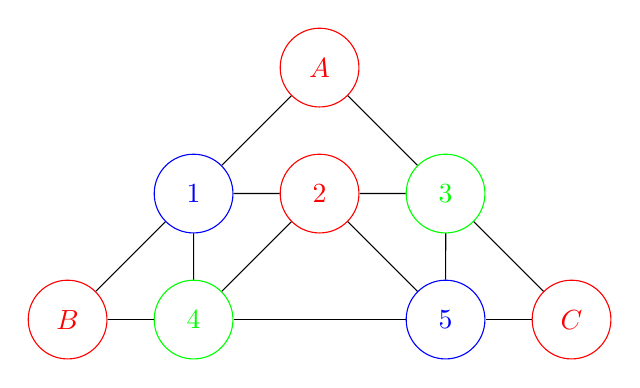
\begin{tikzpicture}[scale=1.6]
		\tikzset{nd/.style={circle, draw=black, minimum width=1cm}};

		\node[nd, red] (a) at (2, 2) {$A$};
		\node[nd, blue] (1) at (1, 1) {$1$};
		\node[nd, red] (2) at (2, 1) {$2$};
		\node[nd, green] (3) at (3, 1) {$3$};
		\node[nd, red] (b) at (0, 0) {$B$};
		\node[nd, green] (4) at (1, 0) {$4$};
		\node[nd, blue] (5) at (3, 0) {$5$};
		\node[nd, red] (c) at (4, 0) {$C$};

		\draw (a) to (1);
		\draw (a) to (3);

		\draw (1) to (2);
		\draw (1) to (b);
		\draw (1) to (4);

		\draw (2) to (3);
		\draw (2) to (4);
		\draw (2) to (5);

		\draw (3) to (5);
		\draw (3) to (c);

		\draw (b) to (4);

		\draw (4) to (5);

		\draw (5) to (c);


	\end{tikzpicture}
\end{center}


\subsubsection{Couleur de $A$, $B$ et $C$}

Supposons, sans perte de généralité\footnote{Les autres configuration peuvent être obetnue par
permutation des sommets et des couleurs.}, que $C$ est de couleur différente :

\begin{center}
	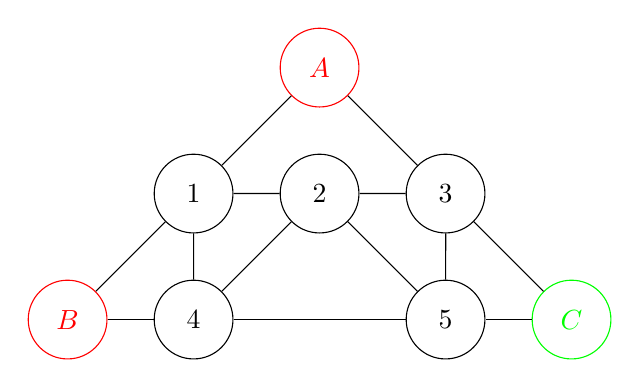
\begin{tikzpicture}[scale=1.6]
		\tikzset{nd/.style={circle, draw=black, minimum width=1cm}};

		\node[nd, red] (a) at (2, 2) {$A$};
		\node[nd] (1) at (1, 1) {$1$};
		\node[nd] (2) at (2, 1) {$2$};
		\node[nd] (3) at (3, 1) {$3$};
		\node[nd, red] (b) at (0, 0) {$B$};
		\node[nd] (4) at (1, 0) {$4$};
		\node[nd] (5) at (3, 0) {$5$};
		\node[nd, green] (c) at (4, 0) {$C$};

		\draw (a) to (1);
		\draw (a) to (3);

		\draw (1) to (2);
		\draw (1) to (b);
		\draw (1) to (4);

		\draw (2) to (3);
		\draw (2) to (4);
		\draw (2) to (5);

		\draw (3) to (5);
		\draw (3) to (c);

		\draw (b) to (4);

		\draw (4) to (5);

		\draw (5) to (c);


	\end{tikzpicture}
\end{center}


La couleur des sommets $3$ et $5$ est alors imposée.

\begin{center}
	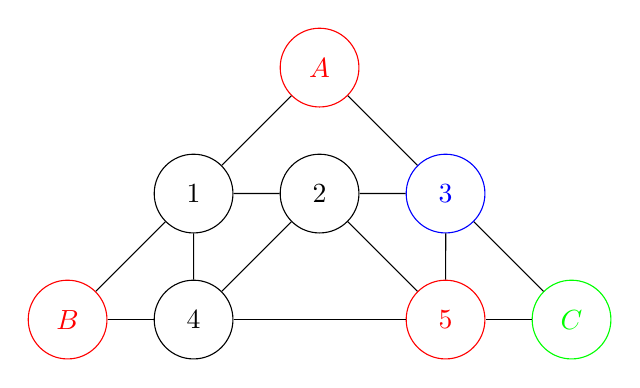
\begin{tikzpicture}[scale=1.6]
		\tikzset{nd/.style={circle, draw=black, minimum width=1cm}};

		\node[nd, red] (a) at (2, 2) {$A$};
		\node[nd] (1) at (1, 1) {$1$};
		\node[nd] (2) at (2, 1) {$2$};
		\node[nd, blue] (3) at (3, 1) {$3$};
		\node[nd, red] (b) at (0, 0) {$B$};
		\node[nd] (4) at (1, 0) {$4$};
		\node[nd, red] (5) at (3, 0) {$5$};
		\node[nd, green] (c) at (4, 0) {$C$};

		\draw (a) to (1);
		\draw (a) to (3);

		\draw (1) to (2);
		\draw (1) to (b);
		\draw (1) to (4);

		\draw (2) to (3);
		\draw (2) to (4);
		\draw (2) to (5);

		\draw (3) to (5);
		\draw (3) to (c);

		\draw (b) to (4);

		\draw (4) to (5);

		\draw (5) to (c);


	\end{tikzpicture}
\end{center}


Ce qui impose les couleurs de $2$ et $4$ et on ne peut pas colorer $1$.

\begin{center}
	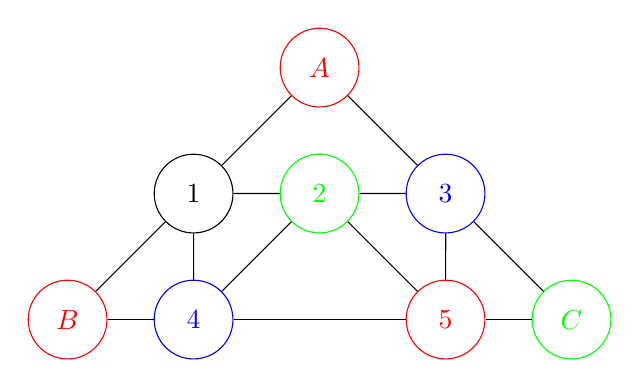
\begin{tikzpicture}[scale=1.6]
		\tikzset{nd/.style={circle, draw=black, minimum width=1cm}};

		\node[nd, red] (a) at (2, 2) {$A$};
		\node[nd] (1) at (1, 1) {$1$};
		\node[nd, green] (2) at (2, 1) {$2$};
		\node[nd, blue] (3) at (3, 1) {$3$};
		\node[nd, red] (b) at (0, 0) {$B$};
		\node[nd, blue] (4) at (1, 0) {$4$};
		\node[nd, red] (5) at (3, 0) {$5$};
		\node[nd, green] (c) at (4, 0) {$C$};

		\draw (a) to (1);
		\draw (a) to (3);

		\draw (1) to (2);
		\draw (1) to (b);
		\draw (1) to (4);

		\draw (2) to (3);
		\draw (2) to (4);
		\draw (2) to (5);

		\draw (3) to (5);
		\draw (3) to (c);

		\draw (b) to (4);

		\draw (4) to (5);

		\draw (5) to (c);


	\end{tikzpicture}
\end{center}


\subsubsection{Degré des sommets dans le gadget étendu}

Dans le graphe ci dessus, tous les sommets sont de degré 4, sauf $A$, $B$ et $C$. Le gadget étendu
est construit en répétant le graphe ci-dessus $n$ fois et de telle sorte que $\forall k \in 1, \dots,
n-1$, $C_{k-1} = B_k$. Le degré des sommets $B_k$, $k \in 1, \dots, n$ est donc de $4$. Donc tous
les sommets sont de degré $4$ sauf $B_0, C_{n-1}, A_k$, $k \in 0 \dots n-1$ qui sont de degré $2$.

\subsubsection{Graphe planaire}

La brique élémentaire est planaire, et la répétition du motif n'entraînant pas d'intersection, le
graphe final est planaire.

\subsubsection{Couleur de $A_n$, $B_0$ et $C_{n-1}$}

L'hypothèse est vérifié pour $n=1$, on la suppose vraie pour $n=m$, qu'en est il de la $m+1^e$
opération ?

Puisque $C_{m-1}$ est rouge, l'hypothèse est vraie au rang $m$, alors $B_m$ est rouge aussi puisque
les deux sommets sont confondu. Ce dernier appartenant à une clique de taille 3, il n'existe qu'une
possibilité pour colorer ses sommets voisins (à permutation des couleurs près).

\begin{center}
	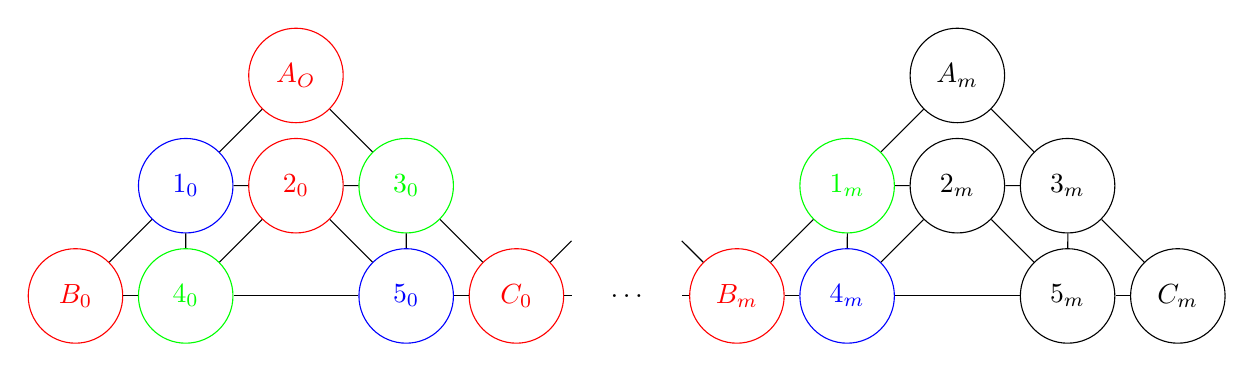
\begin{tikzpicture}[scale=1.4]
		\tikzset{nd/.style={circle, draw=black, minimum width=1.2cm}};

		\node[nd, red] (a0) at (2, 2) {$A_O$};
		\node[nd, blue] (10) at (1, 1) {$1_0$};
		\node[nd, red] (20) at (2, 1) {$2_0$};
		\node[nd, green] (30) at (3, 1) {$3_0$};
		\node[nd, red] (b0) at (0, 0) {$B_0$};
		\node[nd, green] (40) at (1, 0) {$4_0$};
		\node[nd, blue] (50) at (3, 0) {$5_0$};
		\node[nd, red] (c0) at (4, 0) {$C_0$};
		\node (rien0) at (5,0) {$\dots$};
		\node[nd] (a1) at (8, 2) {$A_m$};
		\node[nd, green] (11) at (7, 1) {$1_m$};
		\node[nd] (21) at (8, 1) {$2_m$};
		\node[nd] (31) at (9, 1) {$3_m$};
		\node[nd, red] (b1) at (6, 0) {$B_m$};
		\node[nd, blue] (41) at (7, 0) {$4_m$};
		\node[nd] (51) at (9, 0) {$5_m$};
		\node[nd] (c1) at (10, 0) {$C_m$};
	

		\draw (a0) to (10);
		\draw (a0) to (30);
		\draw (10) to (20);
		\draw (10) to (b0);
		\draw (10) to (40);
		\draw (20) to (30);
		\draw (20) to (40);
		\draw (20) to (50);
		\draw (30) to (50);
		\draw (30) to (c0);
		\draw (b0) to (40);
		\draw (40) to (50);
		\draw (50) to (c0);

		\draw (c0) to (4.5, 0.5);
		\draw (c0) to (4.5, 0);

		\draw (b1) to (5.5, 0.5);
		\draw (b1) to (5.5, 0);

		\draw (a1) to (11);
		\draw (a1) to (31);
		\draw (11) to (21);
		\draw (11) to (b1);
		\draw (11) to (41);
		\draw (21) to (31);
		\draw (21) to (41);
		\draw (21) to (51);
		\draw (31) to (51);
		\draw (31) to (c1);
		\draw (b1) to (41);
		\draw (41) to (51);
		\draw (51) to (c1);


	\end{tikzpicture}
\end{center}


Le sommet $2_m$ est obligatoirement de couleur rouge et donc $5_m$ et de couleur, ce qui impose la
coloration bleue de $3_m$.

\begin{center}
	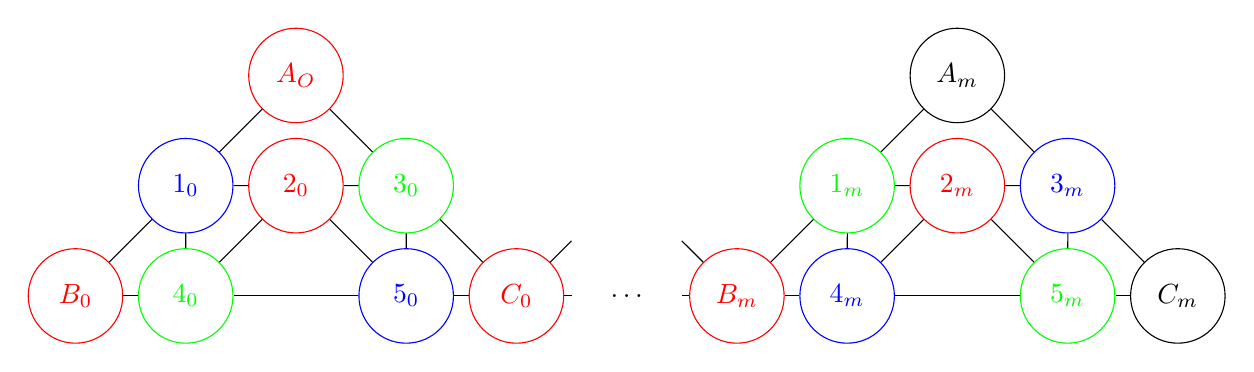
\begin{tikzpicture}[scale=1.4]
		\tikzset{nd/.style={circle, draw=black, minimum width=1.2cm}};

		\node[nd, red] (a0) at (2, 2) {$A_O$};
		\node[nd, blue] (10) at (1, 1) {$1_0$};
		\node[nd, red] (20) at (2, 1) {$2_0$};
		\node[nd, green] (30) at (3, 1) {$3_0$};
		\node[nd, red] (b0) at (0, 0) {$B_0$};
		\node[nd, green] (40) at (1, 0) {$4_0$};
		\node[nd, blue] (50) at (3, 0) {$5_0$};
		\node[nd, red] (c0) at (4, 0) {$C_0$};
		\node (rien0) at (5,0) {$\dots$};
		\node[nd] (a1) at (8, 2) {$A_m$};
		\node[nd, green] (11) at (7, 1) {$1_m$};
		\node[nd, red] (21) at (8, 1) {$2_m$};
		\node[nd, blue] (31) at (9, 1) {$3_m$};
		\node[nd, red] (b1) at (6, 0) {$B_m$};
		\node[nd, blue] (41) at (7, 0) {$4_m$};
		\node[nd, green] (51) at (9, 0) {$5_m$};
		\node[nd] (c1) at (10, 0) {$C_m$};
	

		\draw (a0) to (10);
		\draw (a0) to (30);
		\draw (10) to (20);
		\draw (10) to (b0);
		\draw (10) to (40);
		\draw (20) to (30);
		\draw (20) to (40);
		\draw (20) to (50);
		\draw (30) to (50);
		\draw (30) to (c0);
		\draw (b0) to (40);
		\draw (40) to (50);
		\draw (50) to (c0);

		\draw (c0) to (4.5, 0.5);
		\draw (c0) to (4.5, 0);

		\draw (b1) to (5.5, 0.5);
		\draw (b1) to (5.5, 0);

		\draw (a1) to (11);
		\draw (a1) to (31);
		\draw (11) to (21);
		\draw (11) to (b1);
		\draw (11) to (41);
		\draw (21) to (31);
		\draw (21) to (41);
		\draw (21) to (51);
		\draw (31) to (51);
		\draw (31) to (c1);
		\draw (b1) to (41);
		\draw (41) to (51);
		\draw (51) to (c1);


	\end{tikzpicture}
\end{center}


On a alors $A_m$ et $C_m$ qui sont de couleur rouge, la propriété est donc démontrée.

\begin{center}
	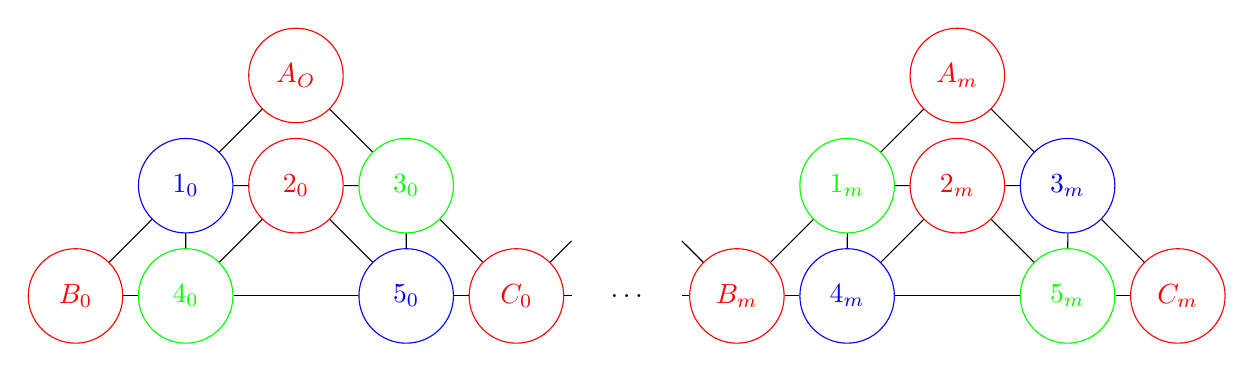
\begin{tikzpicture}[scale=1.4]
		\tikzset{nd/.style={circle, draw=black, minimum width=1.2cm}};

		\node[nd, red] (a0) at (2, 2) {$A_O$};
		\node[nd, blue] (10) at (1, 1) {$1_0$};
		\node[nd, red] (20) at (2, 1) {$2_0$};
		\node[nd, green] (30) at (3, 1) {$3_0$};
		\node[nd, red] (b0) at (0, 0) {$B_0$};
		\node[nd, green] (40) at (1, 0) {$4_0$};
		\node[nd, blue] (50) at (3, 0) {$5_0$};
		\node[nd, red] (c0) at (4, 0) {$C_0$};
		\node (rien0) at (5,0) {$\dots$};
		\node[nd, red] (a1) at (8, 2) {$A_m$};
		\node[nd, green] (11) at (7, 1) {$1_m$};
		\node[nd, red] (21) at (8, 1) {$2_m$};
		\node[nd, blue] (31) at (9, 1) {$3_m$};
		\node[nd, red] (b1) at (6, 0) {$B_m$};
		\node[nd, blue] (41) at (7, 0) {$4_m$};
		\node[nd, green] (51) at (9, 0) {$5_m$};
		\node[nd, red] (c1) at (10, 0) {$C_m$};
	

		\draw (a0) to (10);
		\draw (a0) to (30);
		\draw (10) to (20);
		\draw (10) to (b0);
		\draw (10) to (40);
		\draw (20) to (30);
		\draw (20) to (40);
		\draw (20) to (50);
		\draw (30) to (50);
		\draw (30) to (c0);
		\draw (b0) to (40);
		\draw (40) to (50);
		\draw (50) to (c0);

		\draw (c0) to (4.5, 0.5);
		\draw (c0) to (4.5, 0);

		\draw (b1) to (5.5, 0.5);
		\draw (b1) to (5.5, 0);

		\draw (a1) to (11);
		\draw (a1) to (31);
		\draw (11) to (21);
		\draw (11) to (b1);
		\draw (11) to (41);
		\draw (21) to (31);
		\draw (21) to (41);
		\draw (21) to (51);
		\draw (31) to (51);
		\draw (31) to (c1);
		\draw (b1) to (41);
		\draw (41) to (51);
		\draw (51) to (c1);


	\end{tikzpicture}
\end{center}


De manière moins visuelle et plus concise, on a démontré que pour colorer une brique élémentaire du
schéma, il faut que les sommets $A$, $B$ et $C$ aient la même couleur. Dans la dernière brique du
schéma, la couleur de $B$ est fixée (expliqué précédemment), ce qui fixe la couleur de $A$ et de
$C$.

\subsubsection{Coloration possible du gadget étendu}

Procédons par récurrence : nous avons démontré que l'hypothèse est vraie au rang $0$. On la suppose
vraie au rang $m$. On a alors une coloration du gadget étendu telle que $A_k, B_0, C_{m-1}$, $k \in
0, \dots, m-1$ ont la même couleur. 

Au rang $m+1$, la couleur de $A_m$ est $C_m$ est fixée et est la même que $B_0$ et tous les $A_k$,
or $B_m$ est confondu avec $C_{m-1}$ donc $B_m$ est de la même couleur que les sommets précédents.
Or si tous les sommets ont la même couleur, il existe une coloration possible de la dernière brique
élémentaire et donc une coloration du gadget étendu au rang $m$. L'hypothèse est donc vérifiée.

\subsection{$NP$-complétude de la 3-coloration d'un graphe dont les sommets sont de degré inférieur
ou égal à 4}

Soit $G$ un graphe planaire quelconque. Pour tous les sommets $i$ de $G$ de dégré strictement $d
>4$, on réalise la transformation suivante pour obtenir $H$ : on sélectionne $z = d-3$ arêtes sortant de
$i$ et on les supprime, $i$ est alors confondu avec le sommet $B_0$ d'un gadget étendu au rang $z-1$.
les sommets adjacents aux arêtes sélectionnées sont reliés aux sommets $C_{z-2}$ et$A_k$, $k=1, \dots,
z-2$.

On transforme alors $G$ en graphe planaire dont tous les sommets ont un degré inférieur ou égal à
$4$. De plus une 3-coloration pour $G$ est une 3-coloration pour $H$ puisqu'il est possible de colorer
le gadget en fixant la couleur des sommets $A_k$ et $C_{z-2}$ à celle de $B_0$.

Inversement une 3-coloration de $H$ est une 3-coloration de $G$ puisque les sommets du gadget étendu
auxquels sont reliés les sommets adjecents à $i$ dont de la même couleur que $i$, donc lors de la
suppression des gadgets étendus, les sommets adjacents à $i$ seront d'une couleur différente de
celle de $i$.

Supposons à présent qu'il existe un algorithme polynomial résolvant 3-COLOR-PLAN(G) tel que les
sommets de $G$ ont un degré inférieur ou égal à $4$. La transformation d'un graphe planaire $H$ dont
les sommets sont de degrés quelconque est en temps polynomial, donc il existerait un algorithme
résolvant 3-COLOR-PLAN. Or ce dernier est $NP$-complet, donc l'existence de cet algorithme n'est
vraie que si $P = NP$.

\subsubsection{Graphe planaire dont les sommets sont de degré inférieur ou égal à 2}

Tous ces graphes sont 3-coloriable.

\section{Exercice 13 - Sur le problème de la coloration sur liste}

\subsection{$(=k-k)$-List coloring}

Considérons un graphe $H(X,Y,E)$ biparti construit de la façon suivante :
\begin{itemize}
	\item X est l'ensemble des sommets de $G$
	\item Y est l'ensemble des couleurs appartenant à au moins une liste $L$
	\item soient $x \in X$ et $y \in Y$, $(x,y) \in E$ si et seulement si $y \in L(x)$
\end{itemize}

On recherche alors un couplage parfait dans $H$. La résolution de ce problème nous donne une
solution au problème de la coloration par liste dans la mesure où, si l'on trouve un couplage
parfait, tous les sommets ont une couleur différente\footnote{Il peut exister des solutions de
coloration par liste qui ne donnent pas lieu à un couplage parfait dans $H$, mais celà importe peu
puisque l'on cherche à démontrer que pour ce problème il existe toujours un couplage parfait dans
$H$ et donc une $k-$liste-coloration pour $G$.}

Par définition du problème, on a $n$ listes contenant exactement $k$ couleurs, chaque couleur
apparaissant dans au plus $k$ listes. Le nombre de couleurs est alors minoré par le nombre de
sommets et la relation suivante est vérifiée : $$
|\bigcup_{v \in V'} L(v)| \geq |V'|, \quad \forall V' \subset V $$
Donc d'après le théorème de Hall, il existe un système de représentants distincts $c_v^\in L(v), v
\in V$, autrement dit on peut trouver un couplage parfait dans le graphe $H$.

\subsection{Instances particulières}

\subsubsection{$(2,\infty)-$List coloring}

Nous supposerons par la suite que chaque liste est de taille $2$. On cherchera à montrer que la
formule $\phi_e$ est satisfaite par $\phi$ ssi la fonction $f$ est localement valide sur l'arête
$e$, ainsi si $f$ est valide localement sur toutes les arêtes de $G$, $f$ est alors une
2-liste-coloration de $G$. Or 2-SAT étant polynomial et la réduction de $(2, \infty)$-list coloring
vers 2-SAT se faisant en $O(E)$, le problème initial est polynomial.

Dans un premier temps, cherchons à montrer que $\phi_e$ satisfait par $\phi \Rightarrow f$ valide
localement.

Si $\phi$ satisfait $\phi_e$, $\phi_e$ est vraie, listons les cas possibles : \begin{itemize}
	\item $c_u^1 = c_v^1, c_u^2 = c_v^2$ : $\phi_e$ est vraie implique $x_u \not = x_v$ et donc chaque
		sommet de $e$ de couleur différente.
	\item $c_u^1 = c_v^2, c_u^2 = c_v^1$ : $\phi_e$ est vraie implique $x_u = x_v$ et donc chaque
		sommet de $e$ de couleur différente.
	\item $c_u^1 = c_v^1, c_u^2 \not = c_v^2$ : $\phi_e$ est vraie implique qu'une seule ou aucune des
		deux variables doit être vraie et donc chaque somme de $e$ a une couleur différente.
	\item ...
\end{itemize}

De la même manière on peut énumérer les cas et vérifier que si $f$ et valide localement alors
$\phi_e$ est vraie.

On a donc $\phi_e$ est satisfait par $\phi$ si et seulement si $f$ est valide localement et donc
comme expliqué précédemment, $(2, \infty)$-list coloring se résout en temps polynomial.

\subsubsection{$(\infty, 2)-$List coloring}

Soit un graphe $G = (V,E)$ et une collection de listes $L(v), v \in V$ tels que chaque couleur
apparait au plus dans 2 listes. Pour chaque sommet auquel est associée une liste de couleur de
taille $1$, on colore alors le sommet en question et on supprime cette couleur de la liste de ses
voisins. On répète alors cette opération jusqu'à ce que l'on obtienne un ensemble de sommets dont
les listes sont de taille inférieure ou égale à 2\footnote{Il est aussi possible d'arriver à une
contradiction, dans ce cas, le graphe donné n'est pas $(\infty, 2)$-coloriable par liste.} On a
alors une instance de $(2,2)-$list-coloring et comme la recherche d'un couplage parfait se fait en
temps polynomial, la solution de cette instance se trouve en temps polynomial. L'ensemble des
transformation effectué ci-dessus est polynomial, donc $(\infty, 2)-$list-coloring est polynomial.

\subsection{$NP-$Complétude}

\subsubsection{Validité de l'instance construite}

Vérifions les conditions énoncées une à une :
\begin{itemize}
	\item chaque couleur apparait au plus dans 3 listes puisque à chaque variable sont associées deux
		couleurs, or chaque variable apparaissant au plus dans trois clauses (deux fois négativement et
		un fois positivement), on a alors $x$ apparaissant $L(x)$ et dans $L(c)$ une fois chacune et
		$\bar x$ apparaissant 2 fois dans des $L(c)$ différents et un fois dans $L(x)$ donc trois fois en tout.
	\item on voit immédiatement que $|L(v)| \leq 3$ 
\end{itemize}

\subsubsection{$\phi$ satisfiable $\Rightarrow$ $G$ est list coloriable}

Supposons que $f$ est une liste coloration de $G$, on pose : $$
\phi(x) = \left \lbrace \begin{array}{rcl}
	true & si & f(x) = x \\
	false & si & f(x) = \bar x 
\end{array}
\right .
$$

Soit une clause $c$, si $f(c) = x$ pour une variable $x$ quelconque. On a alors par définition de
l'instance construite $\neg x \in c$ et puisque $f$ est une coloration, on a aussi $f \not = x$. On
en déduit que $f(x) = \bar x$, donc $\phi$ est faux et $c$ est mis à vrai par la variable $x$. D'un
autre côté si $f(c) = \bar x$, alors il s'agit de $x$ qui est dans $c$ et $c$ est satisfaite par
$x$.

Dans l'autre sens maintenant, on définit $f$ comme suit, si $\phi$ est satisfaite : $$
f(x) = \left \lbrace \begin{array}{rcl}
	x & si & \phi(x) = vrai \\
	\bar x & si & \phi(x) = faux
\end{array}
\right .
$$

et pour chaque clause $c$ , on choisit une variable $x_c$ satisfaisant $c$, on fixe alors : $$
f(c) = \left \lbrace \begin{array}{rcl}
	x_c & si & \phi(x_c) = faux et \neg x_c \in c \\
	\bar x_c & si & \phi(x_c) = vrai et x_c \in c
\end{array} \right .
$$

$f$ définit alors une coloration valide.

Les preuves ont été trouvée dans l'article suivant :
\emph{Algorithmic complexity of list colorings}
de Jan Kratochvil et Zsolt Tuzab.
